\documentclass{beamer}
\mode<presentation>
{
\usetheme{Frankfurt}
\setbeamercovered{transparent}
}
\usepackage[russian]{babel}
\usepackage[utf8]{inputenc}

\usepackage{mathptmx}
\usepackage{graphics}
\usepackage[scaled=.90]{helvet}
\usepackage{courier}
\usepackage[T1]{fontenc}

\usepackage{listings}
\lstset{language=Python, numberstyle=\tiny, keywordstyle=\color{blue},numbers=left,commentstyle=\color{green},
basicstyle=\footnotesize}

% \title{Современные технологии программирования систем управления для задач
% учебной и специальной робототехники.}
\title{Использования файловых систем в пользовательском пространстве для
построения интерфейса управления мобильных роботов и мехатронных устройств}

\author{Кирсанов К.Б.}
\institute[sensorika]
{ИПМ им. Келдыша РАН}

\date{01.04.2013 // Гуманитарные чтения 2013}

\beamerdefaultoverlayspecification{<+->}

\begin{document}

\begin{frame}
\titlepage
\end{frame}

\begin{frame}
\frametitle{Содержание}
\tableofcontents
\end{frame}


\section{Введение}
\begin{frame}
\frametitle{Введение}
Для обеспечения взаимодействия с мехатронными устройствами требуется создание
интерфейсов, как пользовательских (для человека), так и программных (для программ). 
В данной работе рассматривается опыт построения такого интерфейса, на основе абстракции файловой системы.

\end{frame}


\section{Интрефейсы программирования}
\begin{frame}
\frametitle{Интрефейсы программирования}

\begin{itemize}
\item<1> \em{Интерфейс} — совокупность возможностей взаимодействия двух систем,
устройств или программ, определённая их характеристиками, характеристиками соединения, сигналов обмена и т. п.


\item<1> Для обеспечения взаимодействия с мехатронными устройствами требуется
создание интерфейсов, как пользовательских (для человека), так и программных (API -
Application Programming Inteface). 


\item<1> В данной работе рассматривается опыт построения интерфейса,
объединяющего в себа обпа типа, на основе абстракции файловой системы.
\end{itemize}
\end{frame}

\subsection{GUI}
\begin{frame}
\frametitle{GUI}
\framesubtitle{Graphical User Interface}
Графический интерфейс пользователя, благодаря своей наглядности, позволяет
быстроприступить к работе
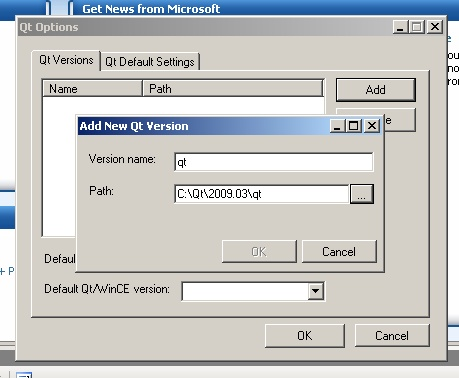
\includegraphics[width=8cm]{button.jpg}
\end{frame}

\begin{frame}
\frametitle{GUI}
Но не всегда\ldots


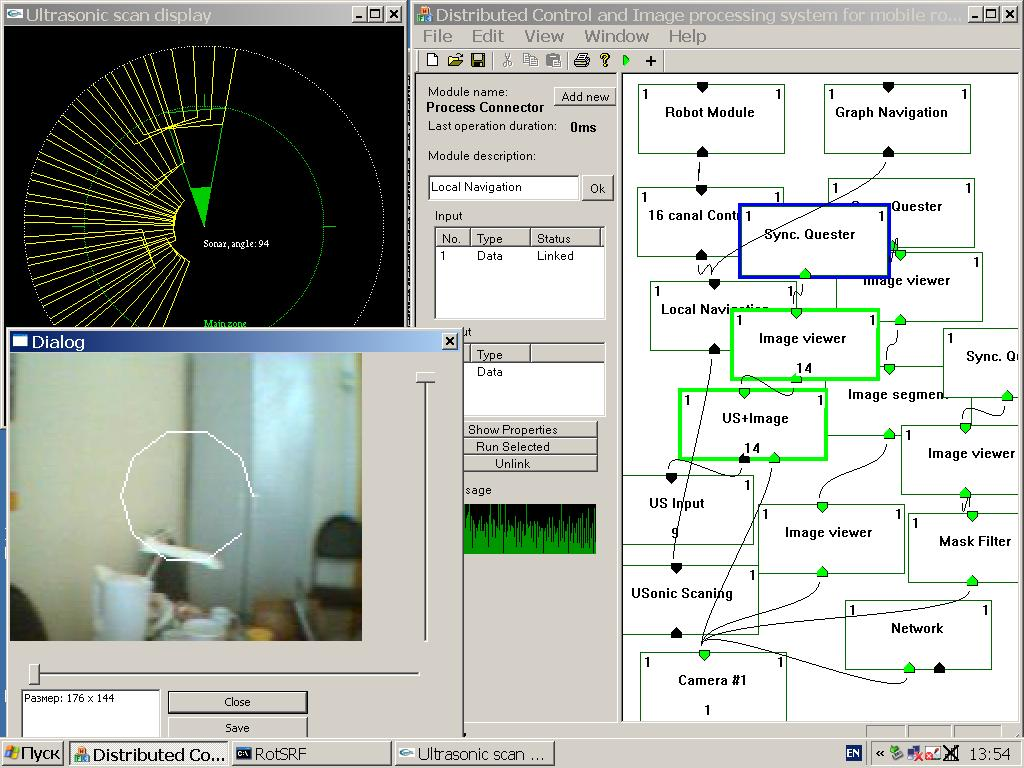
\includegraphics[width=7cm]{hell.jpg}
\end{frame}


\subsection{API}
\begin{frame}
\frametitle{API}
\framesubtitle{Application Programing interface}
API - Application Programing interface
Интерфейс программирования приложений — набор  классов, процедур, функций, структур и констант, предоставляемых приложением (библиотекой, сервисом) для использования во внешних программных продуктах. 
\lstinputlisting{code.py}
\end{frame}

\begin{frame}
\frametitle{API}
\framesubtitle{достоинсва и недостатки, по сравнению с GUI}
\begin{itemize}
  \item<1> API более гибкий
  \item<2> Выше порог вхождения
  \item<2> Требуются специфичные знания, связанные с конкретными языкам,
  платформами и алгоритмами
\end{itemize}

Интерфейсы управления мехатронными устройствами могут быть весьма разнообразны,
причем для программиста, разрабатывающего ПО, программный интерфейс 
(API - Application Programming Interface) фактически становится пользовательским, 
так как для него язык программирования и программа на нем становиться инструментом, 
аналогичном мышке, в руках “обычного” пользователя.

\end{frame}

\section{Новый интрфейс}
\subsection{Файловая система}
\begin{frame}
Файловая система оказывается довольно удачной абстракций для доступа к данным и
состояниям системы управления, т к. с одной стороны работа с ней требует общеизвестных навыков работы 
с файлами и, следовательно, такая абстракция не нуждается в дополнительном изучении, 
а с другой - проста в реализации, что позволяет быстро вводить новые мехатронные устройства в 
работу.


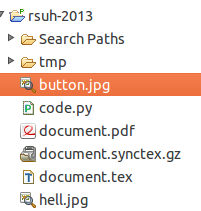
\includegraphics[width=2.3cm]{file.png}
\end{frame}



\subsection{FUSE}
\begin{frame}
\frametitle{FUSE - Filesystem in Userspace}
Для реализации такого рода файловой системы необходимо либо написать собственный
драйвер файловой системы, исполняемый на уроне ядра или же воспользоваться так называемой файловой системой уровня пользователя FUSE


FUSE это модуль для ядер UNIX-подобных операционных систем, обеспечивающий весь
функционал работы с ФС без необходимости предоставления привилегий администратора и внедрения кода в ядро.

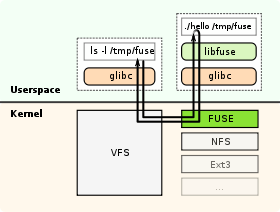
\includegraphics[width=4.3cm]{fuse.png}
\end{frame}

\subsection{Чтение}
\begin{frame}
\frametitle{Чтение}
\begin{itemize}
\item<1> Так, например,  изображение с камеры будет отображаться на файлы
cam1.bmp и cam1.jpg, в форматах bitmap и jpeg соответвенно, что позволит проверить работу камер, 
получить изображение и выполнить другие простейшие операции встроенным в ОС ПО, не прибегая 
программированию или стороннему ПО.
\item<1> Для обеспечения управления, реализумым через запись в файл, такое
простое отображение оказывается уже невозможным, т.к. с одной стороны возникают
коллизии совместного доступа, а с другой тривиальных данных (а только такие и
можно ввести в стандартном текстом редакторе) оказывается явно не доcтаточно.
\end{itemize}
\end{frame}

\subsection{Управление}
\begin{frame}
\frametitle{Управление}
Пускай текущее значение управления ШИМ отображается на файл ./pwm.cmd в виде текста 255, 
что соответсвует максимальному напряжению. Что бы отключить шим достаточно открыть 
данный файл в любом текстовом редакторе, доавить новую строку, и записать в нее 0. 
Таким образом файл примит вид:

\lstinputlisting{code2.py}

Первая строчка обозначает текущее значение шим, а второая - каким значением его
следует подменять. В момент сохранения файла специальное ПО, его и модифицирует программу управления так, 
что бы на ШИМ поступал 0. 
При следующем открытии файла в нем будут те же строки, что позволит корректно его 
модифицировать в дальнейшем.
\end{frame}

\subsection{Программрвоание}
\begin{frame}
\frametitle{Программрование}
Но подмена константой не всегда оказывается достаточной. По этой причине была реализована возможность написания простых программ в том же файле.

\lstinputlisting{code3.py}

Переменной x на каждом витке цикла управления  автоматически присваивается
значение параметра  и, по завершении программы, это значeние и подается на
управление.
\end{frame}


\subsection{Протоколирвоание}
\begin{frame}
\frametitle{Протоколирование}
Отдельно следует упомянуть задачу протоколирования. История(шлейф) состояний отображается на 
соответствующие файлы с расширением .history так, например, файл, в которых
отображается история УЗ измерений имеет следующий вид:

\lstinputlisting{code4.py}


где первый столбец - время измерения, относительно старта системы в секундах, а второй - данные измерений.

\end{frame}

\begin{frame}
\center{Спасибо за внимание}
\end{frame}


\end{document}